\chapter{CNNs results}

\section{Comparing the CNN to the current method}

CNN weitestgehend optimiert und nur noch kleinere Fortschritte hier zu erwarten

Deshalb nun Performance des CNN evaluieren

erst ansehen wie sich simulierte Daten verteilen (Histogramm)

Ratio von gamma zu hadron bekannt und verhält sich wie erwartet

viele korrekt simuliert und doch sehr ähnliche events schwer zu unterscheiden

\begin{figure}
    \centering
    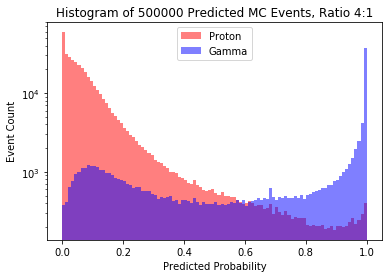
\includegraphics[width=10cm]{Plots/MC_Prediction_Histogram.png}
    \caption{CNN predictions of simulated events}
    \label{fig:histogram_simulated_data}
\end{figure}

histogram vergleich auf echten daten

ähnliche verteilung erwartet nur in der größenordnung unterschiedlich

es stellt sich komplett anderes verhaöten ein

lässt auf missmatch schließen und rückschlüsse auf fehlerhafte ausgangsdaten zulässig

\begin{figure}
    \centering
    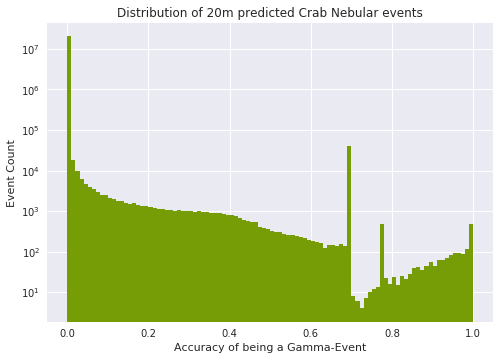
\includegraphics[width=10cm]{Plots/Predicting_real_data.png}
    \caption{CNN predictions of real events}
    \label{fig:histogram_real_data}
\end{figure}

schlussendlich vergleich über theta-plot

erklärung, dass on-off-daten genommen werden und dann die signifikanz der quelle errechnet wird

signifikanz für die messdauer miserabel!

da cnn weitestgehend optimiert, nicht mit optimierung rauszukriegen

\begin{figure}
    \centering
    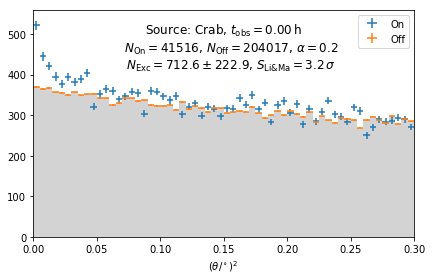
\includegraphics[width=10cm]{Plots/Theta_Plot.png}
    \caption{Theta-Plot for the significance of the crab nebula}
    \label{fig:theta_plot}
\end{figure}


\section{Potential enhancements}

Weitere Verbesserung für das CNN:

Hyperparametersuche unterstützt durch Reinforcementlearning und eigenständiges finden der optimalen Einstellung

3D Convolution über alle nachbarn (hexagonal to 3D)

Einbeziehen der Zeitinformationen (3D Convolution, 4D Convolution, LSTM/RNN)

Verbessern der Monte Carlo Daten:

Missmatches raussieben

Echter Hintergrund verwenden

Klassifizierer verwenden und dann auf vorhergesagten Labels CNN trainieren (kein Missmatch nur Fehlinformationen)
